\newpage
\section{Tinjauan Pustaka}
\subsection{Proses Rekrutmen}
Proses rekrutmen adalah serangkaian langkah yang diambil oleh perusahaan untuk menarik, menilai, dan memilih kandidat yang paling sesuai untuk mengisi posisi yang tersedia. Proses ini biasanya dimulai dengan identifikasi kebutuhan tenaga kerja, diikuti oleh pencarian kandidat melalui berbagai saluran seperti iklan lowongan kerja, agen perekrutan, dan media sosial. Setelah kandidat ditemukan, mereka akan melalui tahap seleksi yang melibatkan penilaian kualifikasi, wawancara, dan tes keterampilan. Akhirnya, keputusan perekrutan dibuat berdasarkan evaluasi menyeluruh dari semua kandidat yang telah melalui proses seleksi. Proses rekrutmen yang efektif tidak hanya memastikan bahwa perusahaan mendapatkan karyawan yang berkualitas, tetapi juga membantu dalam membangun budaya organisasi yang positif dan mendukung tujuan bisnis jangka panjang. \parencite{mathis2017human}

Adapun beberapa faktor yang mempengaruhi keputusan perekrutan meliputi:
\begin{enumerate}
    \item Demografis: usia, gender, latar belakang pendidikan. \parencite{ng2005person}
    \item Pengalaman kerja: jumlah tahun pengalaman dan variasi perusahaan sebelumnya. \parencite{ployhart2006staffing}
    \item Kompetensi teknis dan soft skills: hasil tes keterampilan (skill score), wawancara, dan penilaian kepribadian. \parencite{schmidt1998validity}
    \item Faktor eksternal: jarak tempat tinggal ke kantor sering menjadi pertimbangan dalam retensi. \parencite{hausknecht2009targeted}
    \item Strategi rekrutmen: pendekatan organisasi (job fairs, rekrutmen online, campus hiring) dapat memengaruhi kualitas kandidat. \parencite{breaugh2013employee}.
\end{enumerate}

Berdasarkan studi literatur, faktor-faktor di atas secara signifikan mempengaruhi keputusan perekrutan. Dimana hal tersebut dapat menjadi pertimbangan penting dalam pengembangan model prediktif untuk proses perekrutan.

\subsection{CRISP-DM}
CRISP-DM (Cross-Industry Standard Process for Data Mining) adalah metodologi standar yang digunakan dalam proyek data mining dan analisis data. Metodologi ini terdiri dari enam fase utama yang membantu dalam mengorganisir dan mengelola proyek data secara sistematis. \parencite{chumbar2020crispdm}

\begin{figure}[H]
    \centering
    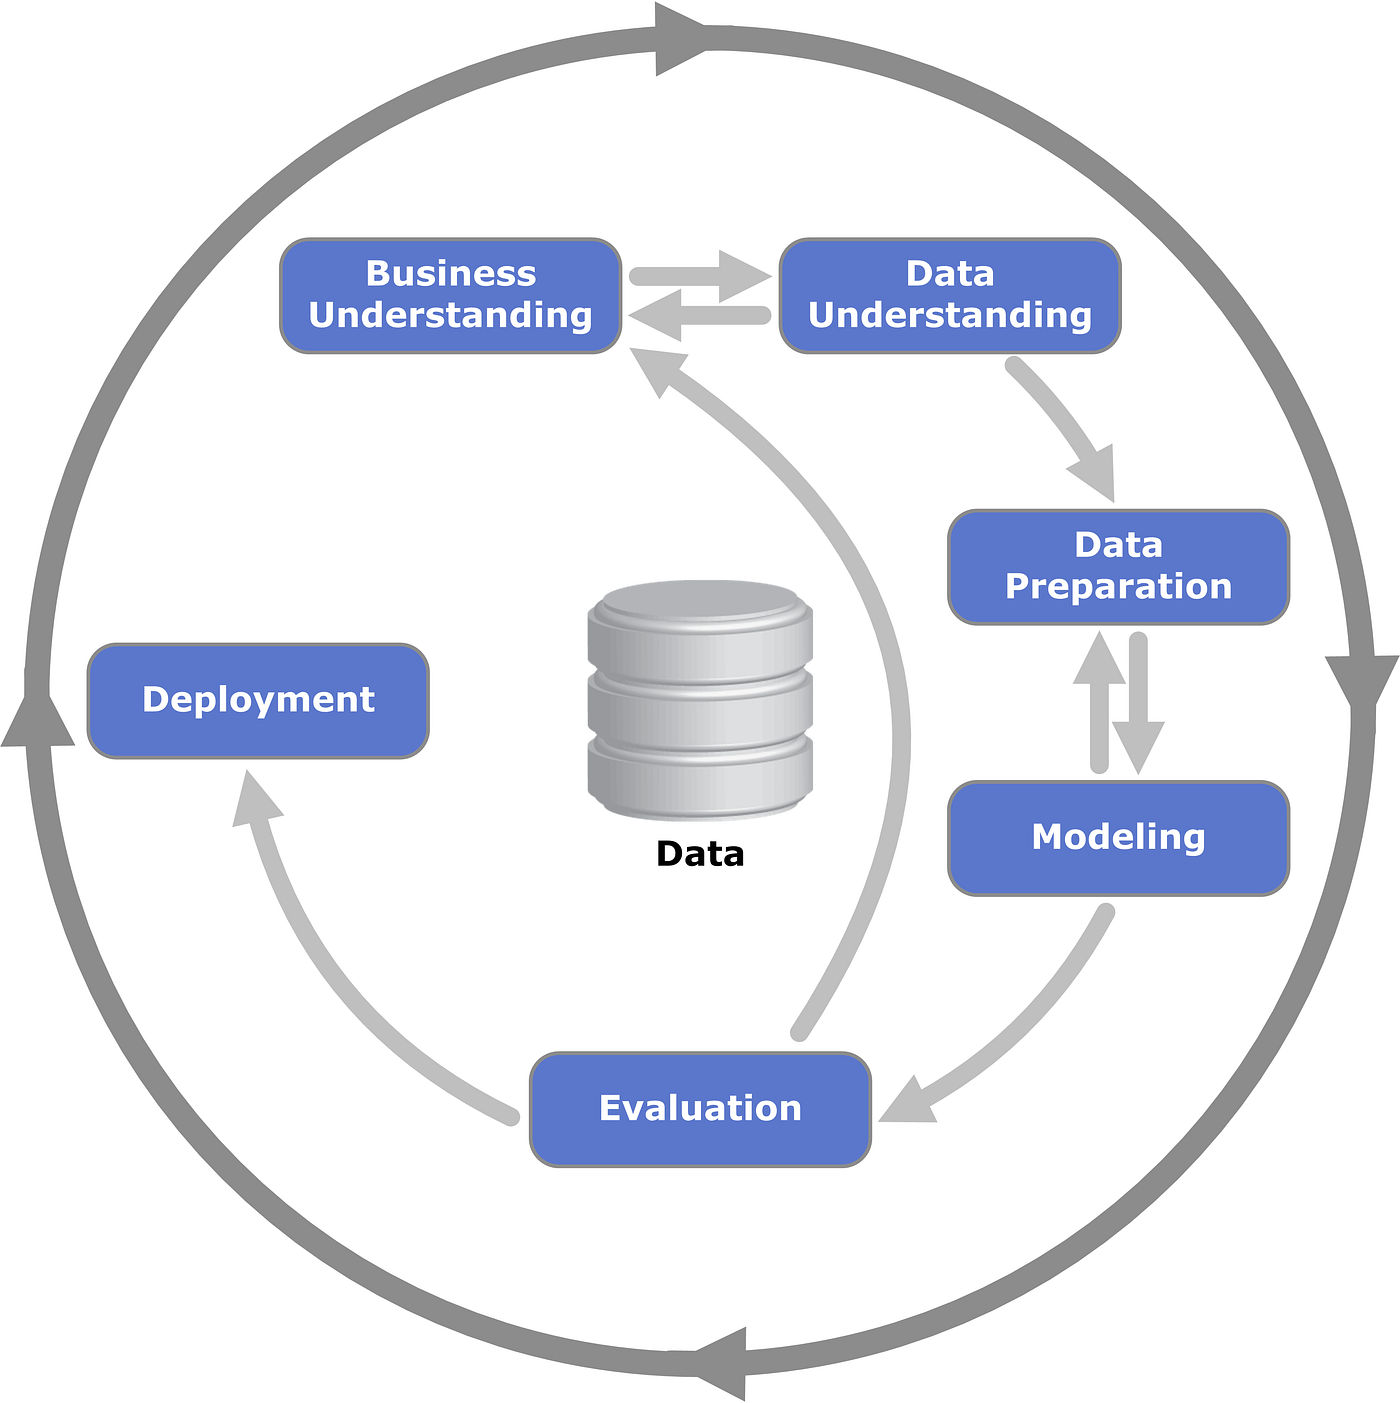
\includegraphics[width=0.4\textwidth]{Gambar/CRISP-DM.png}
    \caption{Alur Kerja CRISP-DM}
    \label{fig:crisp-dm}
\end{figure}

Gambar \ref{fig:crisp-dm} menggambarkan alur kerja CRISP-DM yang terdiri dari enam fase utama, yaitu:
\begin{enumerate}
    \item Business Understanding: Memahami tujuan bisnis dan kebutuhan proyek.
    \item Data Understanding: Mengumpulkan dan memahami data yang tersedia.
    \item Data Preparation: Membersihkan dan mempersiapkan data untuk analisis.
    \item Modeling: Membangun model prediktif menggunakan teknik machine learning.
    \item Evaluation: Mengevaluasi model untuk memastikan bahwa tujuan bisnis tercapai.
    \item Deployment: Menerapkan model dalam lingkungan produksi untuk digunakan dalam pengambilan keputusan bisnis.
\end{enumerate}

\subsection{EDA (Exploratory Data Analysis)}
Exploratory Data Analysis (EDA) adalah proses awal dalam analisis data yang bertujuan untuk memahami karakteristik dan pola dalam dataset. EDA melibatkan berbagai teknik visualisasi dan statistik untuk mengeksplorasi data, mengidentifikasi outlier, dan menemukan hubungan antara variabel. Proses ini sangat penting karena membantu dalam mengarahkan langkah-langkah selanjutnya dalam analisis data, seperti pemilihan fitur dan pemodelan. \parencite{tukey1977exploratory}

\subsection{T-Test}
T-Test adalah metode statistik yang digunakan untuk membandingkan rata-rata dari dua kelompok data. Uji ini membantu menentukan apakah perbedaan antara kedua kelompok tersebut signifikan secara statistik atau hanya terjadi secara kebetulan. T-Test dapat digunakan dalam berbagai konteks, seperti membandingkan hasil tes antara dua kelompok siswa atau mengevaluasi efektivitas dua metode pengajaran yang berbeda. Hasil dari uji T-Test memberikan nilai p-value yang digunakan untuk menilai signifikansi perbedaan antara kedua kelompok. 
%\parencite{de2011introduction}
%rumus t-test
Rumus untuk menghitung nilai T-Test ($t$) adalah sebagai berikut:
\begin{equation}
    t = \frac{\bar{X_1} - \bar{X_2}}{\sqrt{\frac{s_1^2}{n_1} + \frac{s_2^2}{n_2}}}
\end{equation}
Dimana:
\begin{itemize}
    \item $t$ = nilai T-Test
    \item $\bar{X_1}$ = rata-rata kelompok pertama
    \item $\bar{X_2}$ = rata-rata kelompok kedua
    \item $s_1^2$ = varians kelompok pertama
    \item $s_2^2$ = varians kelompok kedua
    \item $n_1$ = ukuran sampel kelompok pertama
    \item $n_2$ = ukuran sampel kelompok kedua
\end{itemize}

Singkatnya uji t-test ini memudahkan kita dalam membandingkan dua kelompok data untuk menentukan apakah ada perbedaan yang signifikan antara keduanya. Apabila p-value lebih kecil dari tingkat signifikansi (misalnya 0,05), maka kita menolak hipotesis nol dan menyimpulkan bahwa ada perbedaan yang signifikan antara kedua kelompok tersebut. Ini berguna apabila fitur numerik ingin dibandingkan terhadap target kategorikal.


\subsection{Chi Square Test}
Chi Square Test adalah metode statistik yang digunakan untuk menguji hubungan antara dua variabel kategorikal. Uji ini membandingkan frekuensi yang diamati dalam setiap kategori dengan frekuensi yang diharapkan jika tidak ada hubungan antara variabel. Hasil dari uji Chi Square memberikan nilai p-value yang digunakan untuk menentukan apakah hubungan antara variabel tersebut signifikan secara statistik. 
% \parencite{agresti2018statistical}

%rumus uji chi square
Rumus untuk menghitung nilai Chi Square ($\chi^2$) adalah sebagai berikut:
\begin{equation}
    \chi^2 = \sum \frac{(O_i - E_i)^2}{E_i}
\end{equation}
Dimana:
\begin{itemize}
    \item $\chi^2$ = nilai Chi Square
    \item $O_i$ = frekuensi yang diamati dalam kategori ke-i
    \item $E_i$ = frekuensi yang diharapkan dalam kategori ke-i
    \item $\sum$ = penjumlahan untuk semua kategori
\end{itemize}

Apabila p-value lebih kecil dari tingkat signifikansi (misalnya 0,05), maka kita menolak hipotesis nol dan menyimpulkan bahwa ada hubungan yang signifikan antara kedua variabel tersebut. Ini berguna apabila fitur kategorikal ingin dibandingkan terhadap target kategorikal.
%\parencite{agresti2018statistical}

\subsection{Standard Scaler}
Standard Scaler adalah teknik normalisasi data yang digunakan untuk mengubah fitur numerik sehingga memiliki rata-rata (mean) nol dan standar deviasi (standard deviation) satu. Proses ini membantu dalam mengurangi skala variabilitas antar fitur, sehingga model machine learning dapat belajar lebih efektif. Standard Scaler sangat berguna ketika fitur-fitur dalam dataset memiliki rentang nilai yang berbeda-beda, karena dapat meningkatkan konvergensi dan kinerja model. 
%\parencite{jain2016feature}
Rumus untuk menghitung nilai yang telah dinormalisasi ($z$) menggunakan Standard Scaler adalah sebagai berikut:

\begin{equation}
    z = \frac{(X - \mu)}{\sigma}
\end{equation}
Dimana:
\begin{itemize}
    \item $z$ = nilai yang telah dinormalisasi
    \item $X$ = nilai asli dari fitur
    \item $\mu$ = rata-rata (mean) dari fitur
    \item $\sigma$ = standar deviasi (standard deviation) dari fitur
    \item $X - \mu$ = selisih antara nilai asli dan rata-rata
    \item $\frac{(X - \mu)}{\sigma}$ = hasil pembagian selisih dengan standar deviasi
\end{itemize}




